# Enhanced Game Theory Chapter

\section{Game Theory}%
\label{sec:game-theory}
\vspace{1cm}
\begin{figure}[h]%
	\label{fig:paradise}
	\centering
	\fcolorbox{black}{white}{
		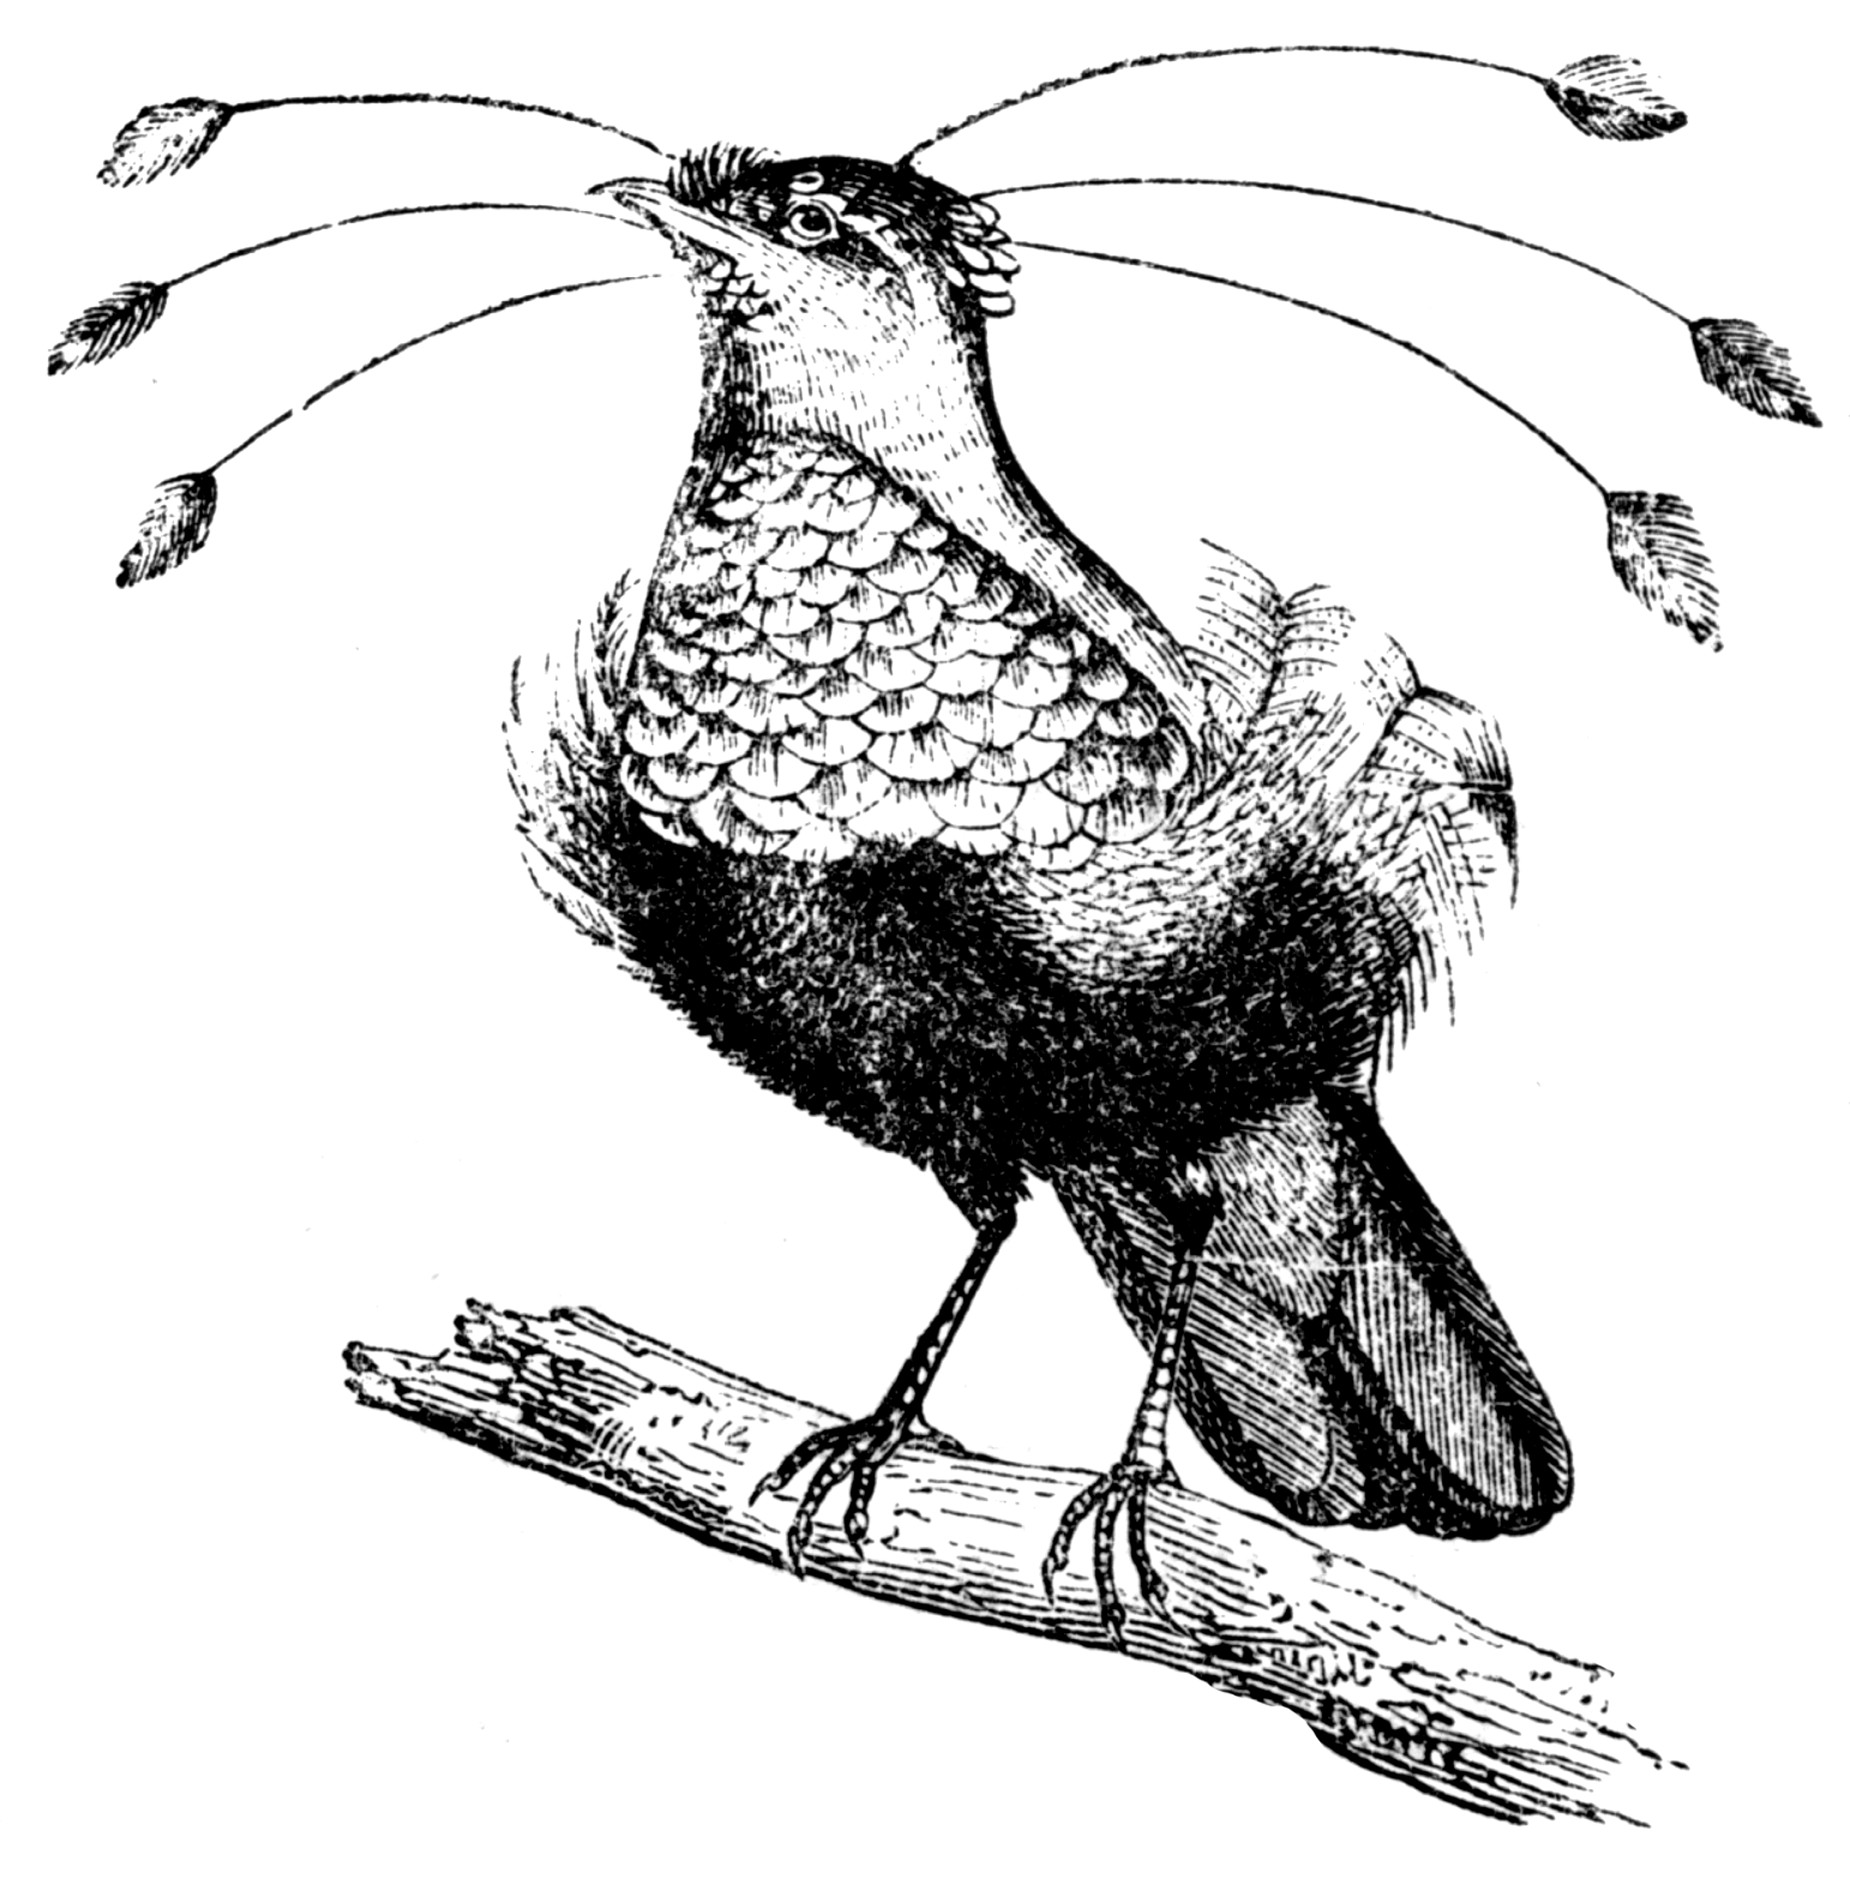
\includegraphics[width=0.3\textwidth]{paradise}
	}
	\caption{Louis Figuier's "Reptiles and Birds" (1869) illustrates the natural adversarial relationships that inspire game-theoretic models.}
\end{figure}
\vspace{1cm}
\noindent The original theoretical formulation of Generative Adversarial Networks, as presented in~\cite{ref:goodfellow-original}, is grounded in \textit{game theory}—the mathematical study of strategic decision-making among rational agents~\cite{ref:myerson}. Throughout this thesis, we focus exclusively on two-player games, using $D$ to represent the discriminator and $G$ to represent the generator. We denote the value function of player $i$ by $V_i$ for $i \in \{D, G\}$.

\begin{definition}%
	\label{def:value-function}
	A \textnormal{\sffamily value function} $V_i$ quantifies the reward (or loss, if negative) for player $i$ in a game as a function of that player's strategic choices.
\end{definition}

\begin{remark}
	In many machine learning contexts, the loss function simply measures the discrepancy between target values $y$ and predictions $\hat{y}$. In GANs, however, the value function is more sophisticated, essentially quantifying uncertainty in the discrimination process.
\end{remark}

Two distinct value functions appear in~\cite{ref:goodfellow-original} (see Section~\ref{sec:two-value}). The first frames the GAN as a \textit{zero-sum game}, while the second formulation does not follow this structure~\cite{ref:gidel-variational-2018}.

\begin{definition}%
	\label{def:zero-sum-game}
	A \textnormal{\sffamily zero-sum game} is one where one player's gain exactly equals the other player's loss. Formally, the players' rewards sum to zero: $V_D + V_G = 0$.
\end{definition}

\begin{remark}
	For this section, we focus on the first value function, treating the GAN algorithm as a zero-sum game between generator and discriminator (see Definitions~\ref{def:generator} and~\ref{def:discriminator}).
\end{remark}

What constitutes an optimal strategy in a zero-sum game? At each turn, what action should a player take to maximize their chances of winning or at least minimize expected loss? The \textit{minimax decision rule} provides a strategy to achieve the best possible outcome when one knows their opponent is actively trying to minimize one's reward.

\begin{definition}
	\label{def:minimax}
	\label{def:minimax-value}
	In a two-player game with players $D$ and $G$, a \textnormal{\sffamily
		minimax decision rule} for $D$ is a strategy that maximizes $D$'s expected
	reward after $G$ has minimized the maximum reward attainable by $D$. The
	\textnormal{\sffamily minimax value} $\overline{V_D}$ for $D$ is the
	largest reward $D$ can secure after $G$ has moved to minimize $D$'s reward:
	\begin{align}
		\overline{V_D} = \min_{G} \max_{D} V_D(D, G).
	\end{align}
\end{definition}

In a game between $D$ and $G$, if $G$ moves first to minimize the reward $D$ can attain, the minimax rule allows $D$ to maximize this reduced reward.

\subsection{Nash Equilibrium and the Prisoner's Dilemma}
\label{sec:nash-dilemma}

The GAN algorithm searches for a \textit{Nash equilibrium} in the parameter space of the discriminator and generator, as discussed in~\cite{ref:goodfellow-2016} and~\cite{ref:goodfellow-2017}.

\begin{definition}
	A \textnormal{\sffamily Nash equilibrium} in an $n$-player game is a
	set of strategies, one for each player, with the property that no
	player can benefit by unilaterally changing their strategy. Let $S_i$ denote the set of strategies for player $i$, and let $S = S_1 \times S_2 \times \cdots \times S_n$ denote the set of strategy profiles. Each strategy profile $s \in S$ combines strategies from all players, dictating each player's action. Let $f_i(s)$ be the payoff to player $i$ under strategy profile $s$. A Nash equilibrium is a strategy profile $s^* = (s_1, s_2, \dots, s_n)$ such that:
	\begin{align}
		f_i(s^*) \geq f_i((s_1, s_2, \dots, s_{-i}, \dots, s_n))
	\end{align}
	for all $i$, where $s_{-i}$ denotes any alternative strategy for player $i$ instead of $s_i$ from $s^*$.
\end{definition}

\begin{remark}
	In a Nash equilibrium, each player's strategy represents an optimal response to the anticipated strategies of other players. A minimax solution to a zero-sum game corresponds to a Nash Equilibrium. Importantly, a Nash equilibrium is not necessarily globally optimal, and a game may have multiple Nash equilibria.
\end{remark}

The \textit{Prisoner's Dilemma} provides an illustrative example of a Nash equilibrium. Originally formulated by Merrill Flood and Melvin Dresher in the 1950s, and later reformulated by Albert W. Tucker in terms of prison sentences (giving it the name \textit{Prisoner's Dilemma})~\cite{ref:poundstone}, this game demonstrates that the globally optimal state may be unattainable in a non-cooperative game. Each player aims to minimize their expected jail time, assuming the other player is doing the same, which prevents them from achieving the global minimum.

\subsubsection{Prisoner's Dilemma}
\label{sec:prisoners-dilemma}

This game involves two players, $D$ and $G$, held separately in police custody with no means of communication. Both have been arrested for a minor crime for which the prosecution has sufficient evidence for conviction. However, prosecutors suspect one of them committed a more serious crime but lack evidence to prove it. The prosecutors offer each player a deal:

\begin{enumerate}
	\item If $D$ defects (accuses $G$ of the serious crime) while $G$ denies involvement, $D$ receives 1 year (as a reward for cooperation) while $G$ receives 5 years (and vice versa);
	\item If both $D$ and $G$ deny involvement in the serious crime, both receive 2 years for the minor crime;
	\item If both $D$ and $G$ accuse each other, both receive 3 years.
\end{enumerate}

\begin{figure}[h]
	\centering%
	\bgroup%
	\def\arraystretch{1.4}
	\begin{tabular}[c]{|c|c|c|}
		\hline
		\diagbox{$D$}{$G$} & Deny   & Defect \\
		\hline
		Deny               & (2, 2) & (5, 1) \\
		\hline
		Defect             & (1, 5) & (3, 3) \\
		\hline
	\end{tabular}
	\egroup
	\caption{Prisoner's Dilemma Payoff Matrix (years in prison for $D$, $G$)}%
	\label{fig:prisoners-matrix}
\end{figure}

Figure~\ref{fig:prisoners-matrix} shows the payoff matrix, with scores representing (years for $D$, years for $G$). Here, $D$ controls the rows and $G$ controls the columns. Although (Deny, Deny) represents the global optimum, it is an unstable state. The state (Defect, Defect) constitutes the Nash equilibrium, as we demonstrate by examining all four possible states:

\begin{enumerate}
	\item \textit{(Deny, Defect):} If $D$ could change their strategy knowing $G$ will defect, $D$ would benefit by switching to defect (reducing their sentence from 5 to 3 years). Thus, this is not a Nash equilibrium. By symmetry, (Defect, Deny) is also not a Nash equilibrium.

	\item \textit{(Deny, Deny):} If both players deny involvement, and $D$ knows $G$ will not change strategy, $D$ can improve their outcome by defecting, changing the state to (Defect, Deny) where $D$ serves only 1 year instead of 2.

	\item \textit{(Defect, Defect):} If both players defect, neither can improve their outcome by unilaterally changing strategy. If $D$ switched to denying, they would serve 5 years instead of 3. The same applies to $G$.
\end{enumerate}

Thus, (Defect, Defect) is the Nash equilibrium—a stable state where neither player has incentive to change strategy unilaterally. Remember that players cannot communicate with each other. As $D$ considers their options, they recognize that $G$ will either defect or deny. To minimize the maximum possible jail time, $D$ should defect, eliminating the worst-case scenario of 5 years. By defecting, the worst outcome for $D$ is 3 years.

Since the minimax strategy in this case does not achieve the global minimum, what implications does this have for the minimax strategy in the GAN algorithm?

\subsection{Derivation of the Value Function}%
\label{sec:derivation}

Now that we've introduced relevant game theory concepts, we can present the GAN algorithm and its constituent neural networks. Let $(\mathcal{X}, p_r)$ be a probability space where $\mathcal{X}$ is a finite space and $p_r$ is the probability distribution over this space. For instance, $\mathcal{X}$ might represent the space of all 8-bit RGB images with height $H$ and width $W$ (i.e., $\mathcal{X} = [0, 255]^{3 \times H \times W}$), and $p_r$ would be the probability distribution assigning mass to regions corresponding to meaningful images (e.g., human faces). Each point in this space represents an image, though most points correspond to meaningless noise.\footnote{Meaningless to human observers, at least.}

The goal of the GAN algorithm is to train a generator $G$, parameterized by $\phi \in \Phi \subset \mathbb{R}^n$, to map random samples $z$ drawn from $(\mathcal{Z}, p_z)$, where $\mathcal{Z} \subset \mathbb{R}^n$, such that $G(z)$ lies in $\mathcal{X}$ in regions where $p_r$ assigns relatively high mass. In practice, $\mathcal{Z} \neq \mathcal{X}$ and $n$ is typically much smaller than $|\mathcal{X}|$~\cite{ref:arjovsky-2017}.

\begin{figure}[H]
	\centering
	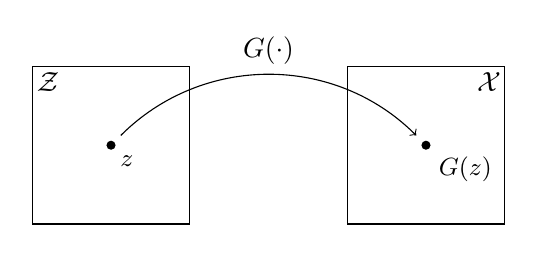
\begin{tikzpicture}
		\node (G) at (3, 2.2) {$G(\cdot)$};
		\draw (0, 0) rectangle +(2, 2);
		\node at (0.2, 1.8) {$\mathcal{Z}$};
		\filldraw (1, 1) circle (0.05cm);
		\node (Z) at (1, 1) {};
		\node (ZZ) at (1.2, 0.8) {\small $z$};
		\draw (4, 0) rectangle +(2, 2);
		\filldraw (5, 1) circle (0.05cm);
		\node (O) at (5, 1) {};
		\node (OO) at (5.5, 0.7) {\small $G(z)$};
		\node at (5.8, 1.8) {$\mathcal{X}$};
		\draw[->] (Z) to [out=45,in=135] (O);
	\end{tikzpicture}
	\caption{The generator $G$ maps noise $z$ to generated data $G(z) \in \mathcal{X}$}%
	\label{fig:g-maps}
\end{figure}

We use a generative model to obtain samples from $\mathcal{X}$ with a specific distribution of values. For instance, if $\mathcal{X}$ is the space of all RGB images and we want images of human faces, we want $G$ to map samples from $\mathcal{Z}$ to regions of $\mathcal{X}$ with RGB values within a narrow range corresponding to facial features.

Initially, $G$ maps $z \in \mathcal{Z}$ to $\mathcal{X}$ randomly. It is from $D$ that $G$ receives gradients to learn. We optimize the discriminator $D$ until it classifies samples sufficiently well—$D$ must learn to assign the correct probability that a sample came from the target distribution. Thus, both $D$ and $G$ learn $p_r$, but from different perspectives.

Let $D$ be a discriminator and $G$ be a generator. Let $V$ be the value function, which depends on the actions (parameterized by $\phi$ and $\theta$) taken by $D$ and $G$:
\begin{align}
	\label{eq:the-original-objective-function}
	V = \mathbb{E}_{x \sim p_r}[\log D_\theta(x)] + \mathbb{E}_{z \sim p_z}[\log{(1 - D_\theta(G_\phi(z)))}].
\end{align}

This value function relates to the one used by the \textit{noise-contrastive estimator} (see~\cite{ref:gutmann-2010}). In the game between $G$ and $D$, each player aims to maximize the minimum reward they can earn, or equivalently, minimize the maximum loss. Generally, a player can minimize their maximum loss by following their minimax decision rule (see Definition~\ref{def:minimax}).

\subsubsection{Derivation of the Value Function from the Perspective of $D$}
\label{sec:derivation-d}

We derive $V$ from $D$'s perspective. We want $D(x)$ to assign mass to $x \in \mathcal{X}$ that approximates the mass assigned by $p_r$. We can achieve this by finding $\theta \in \Theta$ that maximizes the likelihood function:
\begin{align}
	\label{eq:d-1}
	L_{D}^{(1)}(\theta) = \prod_{i=1}^n D(x_i), \quad x_i \sim p_r.
\end{align}

Since this optimization is performed numerically, we maximize the logarithm of the likelihood:
\begin{align}
	\label{eq:d-l1}
	\ell_{D}^{(1)}(\theta) = \log \prod_{i=1}^n D(x_i) = \sum_{i=1}^n \log D(x_i).
\end{align}

Using the logarithm offers two benefits: it is monotone increasing (so any argument maximizing (\ref{eq:d-l1}) also maximizes (\ref{eq:d-1})), and its curvature may improve optimization efficiency by providing steeper gradients.

Simultaneously, since we want $D$ to distinguish generated samples from real samples, we want $D$ to assign low probability (preferably zero) to any generated data point $G(z) = \tilde{x}$. Therefore, for a fixed $G$, $\theta$ must also minimize the following likelihood function:
\begin{align}
	^*L_{D}^{(2)}(\theta) = \prod_{i=1}^n D_\theta(G(z_i)), \quad z_i \sim p_z,
\end{align}

As before, we can minimize $^*L_{D}^{(2)}(\theta)$ by minimizing its logarithm:
\begin{align}
	\label{eq:d-l2} ^*\ell_{D}^{(2)}(\theta) = \log \prod_{i=1}^n D_\theta(G(z_i)) = \sum_{i=1}^n \log D(G(z_i)).
\end{align}

Alternatively, since we're already maximizing (\ref{eq:d-l1}), we can transform (\ref{eq:d-l2}) into a function to be maximized. Specifically, we ask $D$ to maximize:
\begin{align}
	\ell_{D}^{(2)}(\theta) = \sum_{i=1}^n \log{(1 - D_\theta(G_\phi(z_i)))},
\end{align}

since minimizing $D(G(z))$ is equivalent to maximizing $1 - D(G(z))$. Combining $\ell_{D}^{(1)}(\theta)$ and $\ell_{D}^{(2)}(\theta)$, we obtain the following objective function for $D$ to maximize:
\begin{align}
	\sum_{i=1}^n \left( \log D_\theta(x_i) + \log{(1 - D(G(z_i)))} \right).
\end{align}

This is equivalent to maximizing the mean, which, by the law of large numbers, converges to:
\begin{align}
	\label{eq:objective-for-d}
	\mathbb{E}_{x \sim p_r}[\log D(x)] + \mathbb{E}_{z \sim p_z}[\log{(1 - D(G(z)))}]
\end{align}

for sufficiently large $n$. Thus, the GAN algorithm's objective from the discriminator's perspective is to find parameters $\theta$ that maximize (\ref{eq:objective-for-d}).

\subsubsection{Derivation of the Value Function from the Perspective of $G$}%
\label{sec:derivation-g}

From the generator's perspective, we seek $\phi$ that maximizes the likelihood (as defined by a fixed $D$) that a generated sample comes from the target distribution $p_r$. That is, we want $G$ to maximize:
\begin{align}
	^*\ell_G(\phi) = \log\prod_{i=1}^n D(G(z_i)) = \sum_{i=1}^n \log{D(G(z_i))}, \quad z_i \sim p_z.
\end{align}

Alternatively, we can minimize:
\begin{align}
	\ell_G(\phi) = \sum_{i=1}^n \log{(1 - D(G(z_i)))},
\end{align}

which is equivalent to minimizing $\mathbb{E}_{z \sim p_z} \left[\log{(1 - D(G(z)))} \right]$.

\subsubsection{Minimax Value for $D$}

The training objectives for $D$ and $G$ lead to the following formula for the minimax value of $D$:
\begin{align}
	\overline{V_{D}} & = \min_{\phi}\max_{\theta}\left(V_{D}(\theta, \phi) \right)                                                          \\
	                 & = \min_{\phi}\max_{\theta}\left(\mathbb{E}\left[\log{D(x)}\right] + \mathbb{E}\left[\log(1 - D(G(z)))\right] \right)
\end{align}

We solve this in the next section by finding the minimax decision rule and minimax value for $D$ (see Theorem~\ref{theorem:minimax}), which corresponds to finding the Nash equilibrium. However, this is often challenging in practice.

\subsubsection{The Difficulty of Finding a Nash Equilibrium}
\label{sec:difficulty}

Finding a Nash equilibrium is not always straightforward. In fact, the following example shows a tendency to oscillate around an equilibrium. This example was inspired by~\cite{ref:weng-2017}. Let $G$ control $x$ and $D$ control $y$.

\begin{example}
	Let $V(x, y) = xy$ be a value function with the following game:
	\begin{align}
		\min_x\max_y V(x, y) = xy.
	\end{align}

	Since $\frac{\partial V}{\partial x} = y$ and $\frac{\partial V}{\partial y} = x$, we obtain the following updates by following the gradient in the appropriate direction:
	\begin{align}
		x^{(t+1)} \gets x^{(t)} - \eta \cdot y; \\
		y^{(t+1)} \gets y^{(t)} + \eta \cdot x;
	\end{align}
	where $\eta > 0$ is the learning rate. The Nash equilibrium for this game is a pair of strategies $s^* = (s_G, s_D)$. If $G$'s strategy is $s^*_G = (0, 0, 0, \dots)$, then $V(s^*_G, s_D) = 0$ for all $s_D$, meaning $D$ cannot improve the value function. Similarly, if $D$ adopts the same strategy $s^*_D = (0, 0, 0, \dots)$, $G$ cannot improve the value function. Hence, $s^* = (s^*_D, s^*_G)$ with $V(s^*_G, s^*_D) = 0$ is the Nash equilibrium.

	\begin{figure}[H]
		\centering
		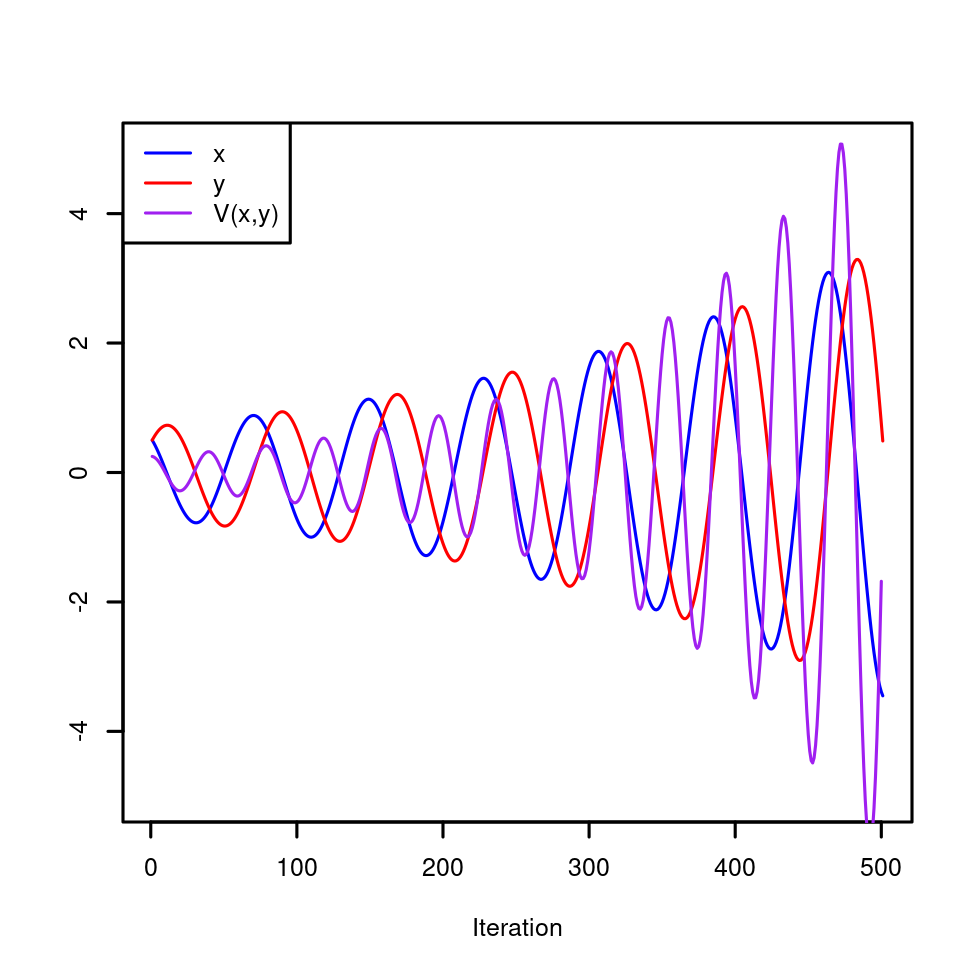
\includegraphics[width=0.6\textwidth]{plot1}
		\caption{Oscillating behavior around the optimal value during gradient-based optimization}
		\label{fig:alternating}
	\end{figure}
\end{example}

As we alternate updates, we observe oscillating behavior as depicted in Figure~\ref{fig:alternating}. This oscillation phenomenon has been observed in GAN training and represents a significant challenge in practice.

\subsubsection{Two Value Functions}%
\label{sec:two-value}

In~\cite{ref:goodfellow-original}, the authors introduced one value function for theoretical discussion but used a different one for actual training to avoid the issues mentioned above. The first value function (equation~\ref{eq:the-original-objective-function}) is difficult to train and often leads to vanishing gradients, leaving the generator with no learning signal. The decoupled objective functions:
\begin{align}
	\label{eq:second-value-function}
	\max_{\theta} \left( \mathbb{E}\left[\log{D_\theta(x)}\right] + \mathbb{E}\left[\log(1 - D_\theta(G_\phi(z)))\right] \right) \\
	\max_{\phi}\mathbb{E}\left[\log(D_\theta(G_\phi(z)))\right]
\end{align}

have the same fixed points as the original formulation but provide stronger gradients with respect to the generator, offering better learning signals. With equation \ref{eq:second-value-function} as the objective functions, the GAN algorithm is no longer a zero-sum game.

\subsection{Generative Adversarial Networks}

The complete GAN algorithm is presented below:

\begin{figure}[H] \centering
	\begin{minipage}{0.95\linewidth}
		\begin{algorithm}[H]
			Let $\eta > 0$ be the learning rate. \\
			Let $T > 0$ be the number of training iterations. \\
			Let $D: \Theta \times \mathcal{X} \mapsto [0, 1]$ \\
			Let $G: \Phi \times \mathcal{Z} \mapsto \mathcal{X}$ \\
			\While {$t < T$} {
				Let $z = \{z_1, \dots, z_m\}$, where each $z_i$ is sampled from $(\mathcal{Z}, p_z)$. \\
				Let $x = \{x_1, \dots, x_m\}$, where each $x_i$ is from the training data. \\
				Update the discriminator's parameters:
				\begin{align*}
					\theta \gets \theta + \eta \cdot \nabla_{\theta} \frac{1}{m} \sum_{i=1}^m \left[ \log{D(x_i)} + \log{(1 - D(G(z_i)))} \right]
				\end{align*}
				Sample a new batch $z = \{z_1, \dots, z_m\}$ from $(\mathcal{Z}, p_z)$. \\
				Update the generator's parameters:
				\begin{align*}
					\phi \gets \phi - \eta \cdot \nabla_{\phi} \frac{1}{m} \sum_{i=1}^m \log{(1 - D(G(z_i)))}
				\end{align*}
			}
			\caption{Generative Adversarial Networks}
			\label{algo:main-algo}
		\end{algorithm}
	\end{minipage}
\end{figure}

In the original paper, the discriminator is optimized $k$ times before each generator update, but typically $k=1$. We've omitted this inner training loop for readability and conceptual clarity.

\subsection{Discussion}

The minimax strategy for $D$ can be understood as follows: if $D$ assumes $G$ has done its best to minimize $D$'s reward, then $D$ should assume $G$ can produce data indistinguishable from real samples. In this case, to minimize loss, $D$ should return $\frac{1}{2}$ for all data points—which happens to be the maximum entropy distribution over the two states (real or synthetic). If $D(x) = \frac{1}{2}$ for all $x$, there is nothing $G$ can do to improve its situation. The next section will demonstrate that $D(x) = \frac{1}{2}$ for all $x$ is indeed the optimal strategy for $D$.

This game-theoretic perspective reveals why GAN training can be challenging: the adversarial nature of the optimization can lead to oscillations around the equilibrium rather than stable convergence. The use of separate objective functions in practice helps mitigate some of these issues but does not eliminate the fundamental challenges of finding a stable equilibrium in high-dimensional parameter spaces.

%%% Local Variables:
%%% mode: latex
%%% TeX-master: "../thesis"
%%% End:
